\documentclass[aspectratio=169,10pt]{beamer}

\usetheme{Madrid}
\usecolortheme{default}
\usefonttheme{professionalfonts}

\usepackage[T1]{fontenc}
\usepackage[utf8]{inputenc}
\usepackage{tikz}
\usepackage{booktabs}
\usetikzlibrary{arrows.meta,positioning,fit,calc,shapes.geometric,shapes.misc,decorations.pathreplacing}

\definecolor{RcaNavy}{RGB}{8,35,70}
\definecolor{RcaNavySoft}{RGB}{28,58,98}
\definecolor{RcaGray}{RGB}{92,99,107}
\definecolor{RcaLightGray}{RGB}{236,239,242}
\definecolor{RcaMidGray}{RGB}{190,197,204}

\setbeamercolor{palette primary}{bg=RcaNavy,fg=white}
\setbeamercolor{palette secondary}{bg=RcaNavySoft,fg=white}
\setbeamercolor{palette tertiary}{bg=RcaNavy,fg=white}
\setbeamercolor{frametitle}{bg=RcaNavy,fg=white}
\setbeamercolor{title}{fg=white,bg=RcaNavy}
\setbeamercolor{normal text}{fg=RcaNavy,bg=white}
\setbeamercolor{structure}{fg=RcaNavy}
\setbeamercolor{block title}{fg=white,bg=RcaNavy}
\setbeamercolor{block body}{fg=RcaNavy,bg=RcaLightGray}
\setbeamertemplate{navigation symbols}{}
\setbeamertemplate{footline}[frame number]
\setbeamertemplate{itemize item}{\color{RcaNavy}\small$\blacktriangleright$}

\tikzset{
  rca/box/.style={
    draw=RcaNavy,
    very thick,
    rounded corners=3pt,
    fill=white,
    align=center,
    text=RcaNavy,
    minimum height=0.78cm,
    inner xsep=6pt,
    inner ysep=4pt,
    font=\small
  },
  rca/softbox/.style={
    draw=RcaMidGray,
    thick,
    rounded corners=3pt,
    fill=RcaLightGray,
    align=center,
    text=RcaNavy,
    minimum height=0.72cm,
    inner xsep=6pt,
    inner ysep=4pt,
    font=\small
  },
  rca/future/.style={
    draw=RcaGray,
    thick,
    dashed,
    rounded corners=3pt,
    fill=white,
    align=center,
    text=RcaGray,
    minimum height=0.72cm,
    inner xsep=6pt,
    inner ysep=4pt,
    font=\small
  },
  rca/db/.style={
    cylinder,
    shape border rotate=90,
    aspect=0.25,
    draw=RcaNavy,
    very thick,
    fill=white,
    align=center,
    text=RcaNavy,
    minimum height=1.15cm,
    minimum width=1.55cm,
    font=\small
  },
  rca/arrow/.style={-{Latex[length=3mm,width=2mm]}, very thick, draw=RcaNavy},
  rca/grayarrow/.style={-{Latex[length=3mm,width=2mm]}, thick, draw=RcaGray},
  rca/dasharrow/.style={-{Latex[length=3mm,width=2mm]}, thick, dashed, draw=RcaGray},
  rca/node/.style={circle, draw=RcaNavy, very thick, fill=white, minimum size=0.78cm, font=\small},
  rca/error/.style={circle, draw=RcaNavy, very thick, fill=RcaLightGray, minimum size=0.82cm, font=\small\bfseries},
  rca/title/.style={font=\bfseries\small, text=RcaNavy, align=center},
  rca/tinylabel/.style={font=\scriptsize, text=RcaGray, align=center}
}

\newcommand{\slidelabel}[1]{\node[font=\scriptsize,text=RcaGray,align=center] {#1};}
\newcommand{\futuretag}{\scriptsize\color{RcaGray}{Future}}
\newcommand{\currenttag}{\scriptsize\color{RcaNavy}{Current}}

\title[OpenStack RCA Copilot]{OpenStack RCA Copilot}
\subtitle{Local-first root cause investigation for OpenStack}
\author{Project Presentation}
\institute{RCA Copilot}
\date{\today}

\begin{document}

\begin{frame}
  \titlepage
\end{frame}

\begin{frame}{Storyline}
\centering
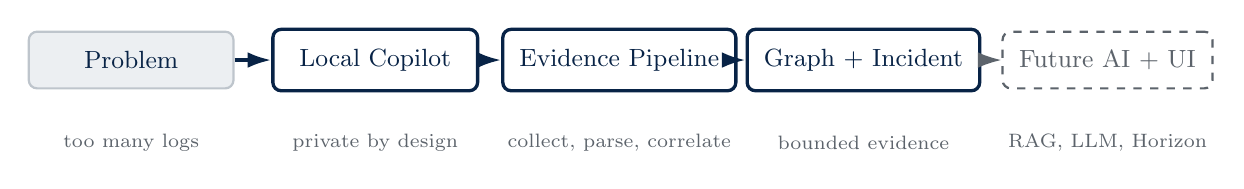
\begin{tikzpicture}[x=1cm,y=1cm]
  \node[rca/softbox,minimum width=2.6cm] (p) at (0,1.6) {Problem};
  \node[rca/box,minimum width=2.6cm] (c) at (3.1,1.6) {Local Copilot};
  \node[rca/box,minimum width=2.6cm] (pipe) at (6.2,1.6) {Evidence Pipeline};
  \node[rca/box,minimum width=2.6cm] (graph) at (9.3,1.6) {Graph + Incident};
  \node[rca/future,minimum width=2.6cm] (ai) at (12.4,1.6) {Future AI + UI};
  \draw[rca/arrow] (p) -- (c);
  \draw[rca/arrow] (c) -- (pipe);
  \draw[rca/arrow] (pipe) -- (graph);
  \draw[rca/dasharrow] (graph) -- (ai);
  \node[rca/tinylabel] at (0,0.55) {too many logs};
  \node[rca/tinylabel] at (3.1,0.55) {private by design};
  \node[rca/tinylabel] at (6.2,0.55) {collect, parse, correlate};
  \node[rca/tinylabel] at (9.3,0.55) {bounded evidence};
  \node[rca/tinylabel] at (12.4,0.55) {RAG, LLM, Horizon};
\end{tikzpicture}
\end{frame}

\begin{frame}{Problem: Logs Are Everywhere}
\centering
\resizebox{\textwidth}{!}{%
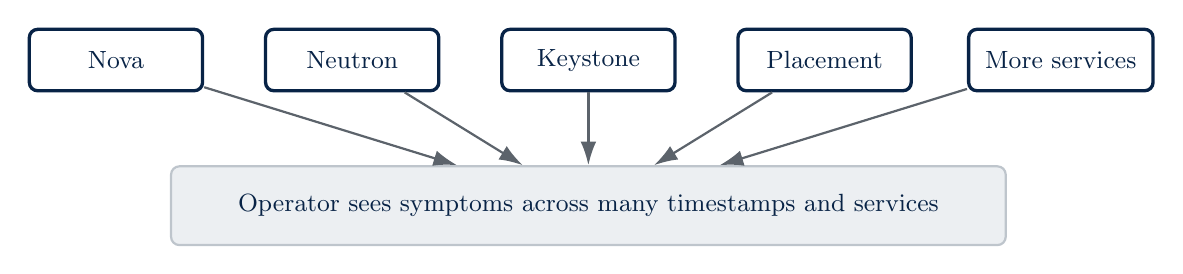
\begin{tikzpicture}[x=1cm,y=1cm]
  \node[rca/box,minimum width=2.2cm] (nova) at (0,2.4) {Nova};
  \node[rca/box,minimum width=2.2cm] (neutron) at (3,2.4) {Neutron};
  \node[rca/box,minimum width=2.2cm] (key) at (6,2.4) {Keystone};
  \node[rca/box,minimum width=2.2cm] (place) at (9,2.4) {Placement};
  \node[rca/box,minimum width=2.2cm] (more) at (12,2.4) {More services};
  \node[rca/softbox,minimum width=10.6cm,minimum height=1.0cm] (op) at (6,0.55) {Operator sees symptoms across many timestamps and services};
  \foreach \a in {nova,neutron,key,place,more}{
    \draw[rca/grayarrow] (\a) -- (op);
  }
\end{tikzpicture}}
\vspace{0.25cm}
\begin{columns}[T,totalwidth=0.88\textwidth]
\column{0.28\textwidth}\centering\small High volume
\column{0.28\textwidth}\centering\small Distributed context
\column{0.28\textwidth}\centering\small Slow manual grep
\end{columns}
\end{frame}

\begin{frame}{RCA Needs Evidence}
\centering
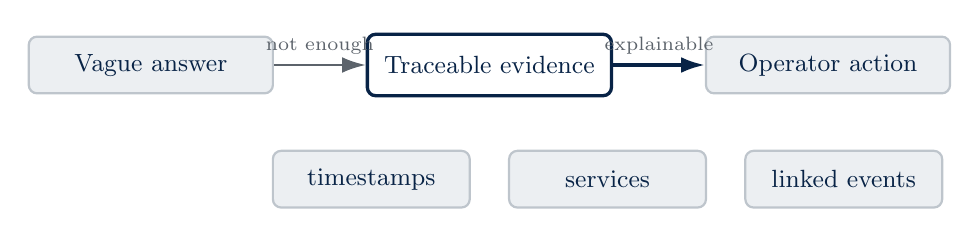
\begin{tikzpicture}[x=1cm,y=1cm]
  \node[rca/softbox,minimum width=3.1cm] (vague) at (1.7,2.2) {Vague answer};
  \node[rca/box,minimum width=3.1cm] (evidence) at (6,2.2) {Traceable evidence};
  \node[rca/softbox,minimum width=3.1cm] (action) at (10.3,2.2) {Operator action};
  \draw[rca/grayarrow] (vague) -- node[above,rca/tinylabel] {not enough} (evidence);
  \draw[rca/arrow] (evidence) -- node[above,rca/tinylabel] {explainable} (action);
  \node[rca/softbox,minimum width=2.5cm] at (4.5,0.75) {timestamps};
  \node[rca/softbox,minimum width=2.5cm] at (7.5,0.75) {services};
  \node[rca/softbox,minimum width=2.5cm] at (10.5,0.75) {linked events};
\end{tikzpicture}
\end{frame}

\begin{frame}{High-Level Concept}
\centering
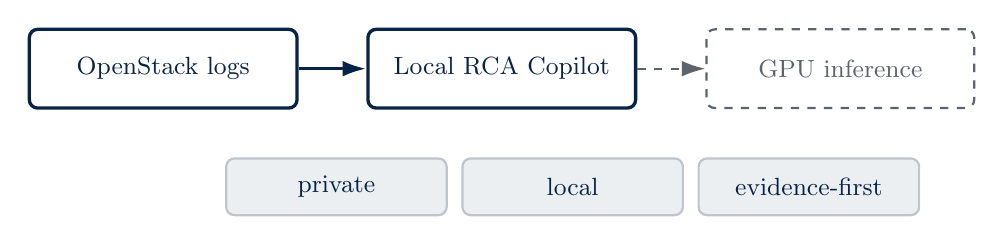
\begin{tikzpicture}[x=1cm,y=1cm]
  \node[rca/box,minimum width=3.4cm,minimum height=1cm] (openstack) at (1.7,2.7) {OpenStack logs};
  \node[rca/box,minimum width=3.4cm,minimum height=1cm] (copilot) at (6,2.7) {Local RCA Copilot};
  \node[rca/future,minimum width=3.4cm,minimum height=1cm] (ai) at (10.3,2.7) {GPU inference};
  \draw[rca/arrow] (openstack) -- (copilot);
  \draw[rca/dasharrow] (copilot) -- (ai);
  \node[rca/softbox,minimum width=2.8cm] at (3.9,1.2) {private};
  \node[rca/softbox,minimum width=2.8cm] at (6.9,1.2) {local};
  \node[rca/softbox,minimum width=2.8cm] at (9.9,1.2) {evidence-first};
\end{tikzpicture}
\end{frame}

\begin{frame}{Two-Machine Vision}
\centering
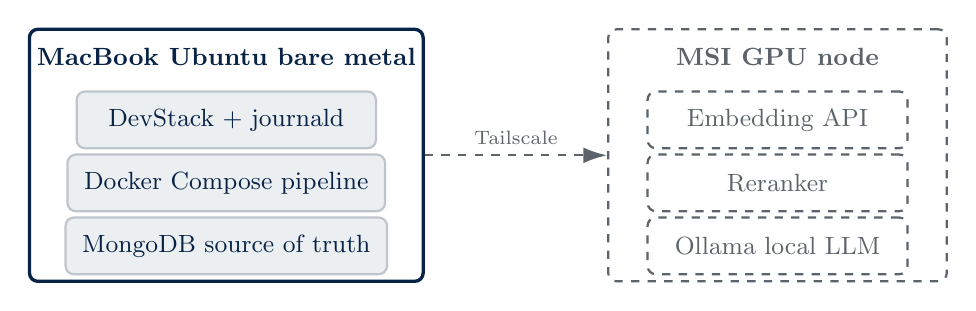
\begin{tikzpicture}[x=1cm,y=1cm]
  \node[rca/box,minimum width=5.0cm,minimum height=3.2cm] (mac) at (3,2.1) {};
  \node[rca/title] at (3,3.35) {MacBook Ubuntu bare metal};
  \node[rca/softbox,minimum width=3.8cm] at (3,2.55) {DevStack + journald};
  \node[rca/softbox,minimum width=3.8cm] at (3,1.75) {Docker Compose pipeline};
  \node[rca/softbox,minimum width=3.8cm] at (3,0.95) {MongoDB source of truth};
  \node[rca/future,minimum width=4.3cm,minimum height=3.2cm] (msi) at (10,2.1) {};
  \node[rca/title,text=RcaGray] at (10,3.35) {MSI GPU node};
  \node[rca/future,minimum width=3.3cm] at (10,2.55) {Embedding API};
  \node[rca/future,minimum width=3.3cm] at (10,1.75) {Reranker};
  \node[rca/future,minimum width=3.3cm] at (10,0.95) {Ollama local LLM};
  \draw[rca/dasharrow] (mac) -- node[above,rca/tinylabel] {Tailscale} (msi);
\end{tikzpicture}
\end{frame}

\begin{frame}{Current Deployment Topology}
\centering
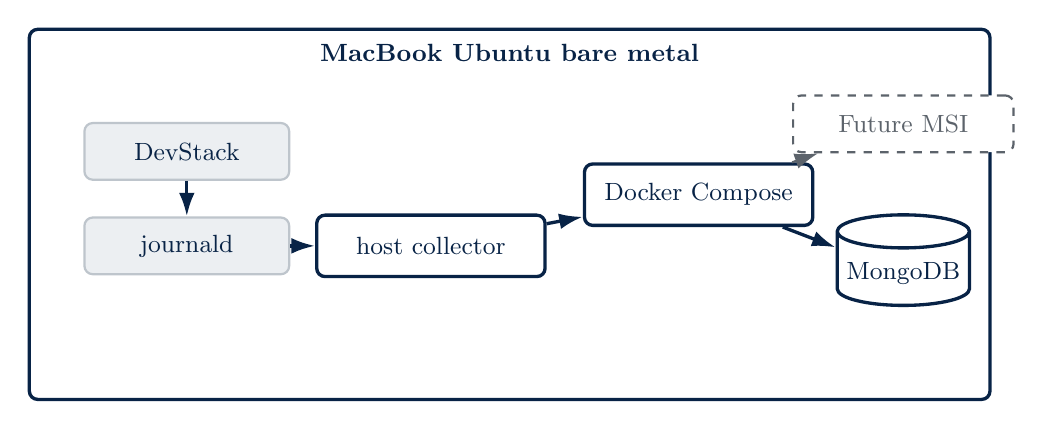
\begin{tikzpicture}[x=1cm,y=1cm]
  \node[rca/box,minimum width=12.2cm,minimum height=4.7cm] at (6,2.3) {};
  \node[rca/title] at (6,4.35) {MacBook Ubuntu bare metal};
  \node[rca/softbox,minimum width=2.6cm] (dev) at (1.9,3.1) {DevStack};
  \node[rca/softbox,minimum width=2.6cm] (jour) at (1.9,1.9) {journald};
  \node[rca/box,minimum width=2.9cm] (col) at (5,1.9) {host collector};
  \node[rca/box,minimum width=2.9cm] (compose) at (8.4,2.55) {Docker Compose};
  \node[rca/db] (mongo) at (11,1.55) {MongoDB};
  \node[rca/future,minimum width=2.8cm] (msi) at (11,3.45) {Future MSI};
  \draw[rca/arrow] (dev) -- (jour);
  \draw[rca/arrow] (jour) -- (col);
  \draw[rca/arrow] (col) -- (compose);
  \draw[rca/arrow] (compose) -- (mongo);
  \draw[rca/dasharrow] (compose) -- (msi);
\end{tikzpicture}
\end{frame}

\begin{frame}{Docker Compose Service Map}
\centering
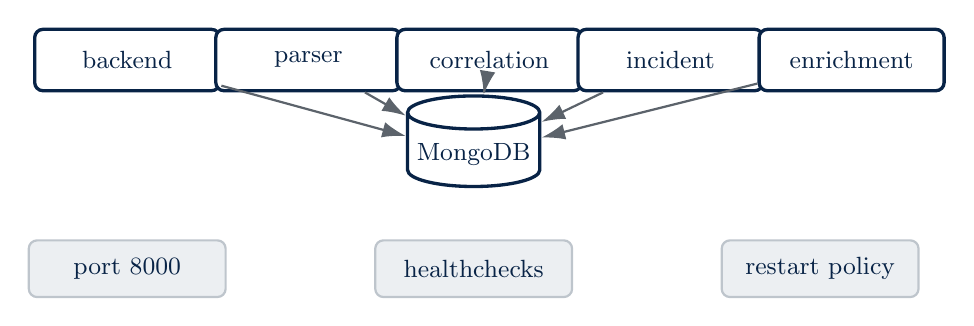
\begin{tikzpicture}[x=1cm,y=1cm]
  \node[rca/db] (mongo) at (6,2.35) {MongoDB};
  \node[rca/box,minimum width=2.35cm] (api) at (1.6,3.55) {backend};
  \node[rca/box,minimum width=2.35cm] (parser) at (3.9,3.55) {parser};
  \node[rca/box,minimum width=2.35cm] (corr) at (6.2,3.55) {correlation};
  \node[rca/box,minimum width=2.35cm] (inc) at (8.5,3.55) {incident};
  \node[rca/box,minimum width=2.35cm] (enrich) at (10.8,3.55) {enrichment};
  \node[rca/softbox,minimum width=2.5cm] at (1.6,0.9) {port 8000};
  \node[rca/softbox,minimum width=2.5cm] at (6,0.9) {healthchecks};
  \node[rca/softbox,minimum width=2.5cm] at (10.4,0.9) {restart policy};
  \foreach \n in {api,parser,corr,inc,enrich}{\draw[rca/grayarrow] (\n) -- (mongo);}
\end{tikzpicture}
\end{frame}

\begin{frame}{MacBook Local Pipeline}
\centering
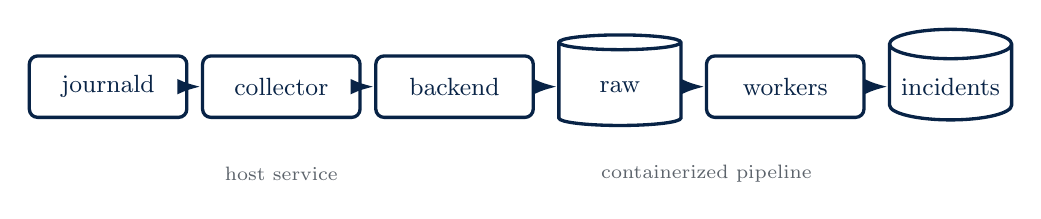
\begin{tikzpicture}[node distance=0.75cm,x=1cm,y=1cm]
  \node[rca/box,minimum width=2.0cm] (j) at (0.8,2.2) {journald};
  \node[rca/box,minimum width=2.0cm] (c) at (3.0,2.2) {collector};
  \node[rca/box,minimum width=2.0cm] (b) at (5.2,2.2) {backend};
  \node[rca/db] (r) at (7.3,2.2) {raw};
  \node[rca/box,minimum width=2.0cm] (p) at (9.4,2.2) {workers};
  \node[rca/db] (i) at (11.5,2.2) {incidents};
  \draw[rca/arrow] (j) -- (c);
  \draw[rca/arrow] (c) -- (b);
  \draw[rca/arrow] (b) -- (r);
  \draw[rca/arrow] (r) -- (p);
  \draw[rca/arrow] (p) -- (i);
  \node[rca/tinylabel] at (3,1.1) {host service};
  \node[rca/tinylabel] at (8.4,1.1) {containerized pipeline};
\end{tikzpicture}
\end{frame}

\begin{frame}{journald Collector Lifecycle}
\centering
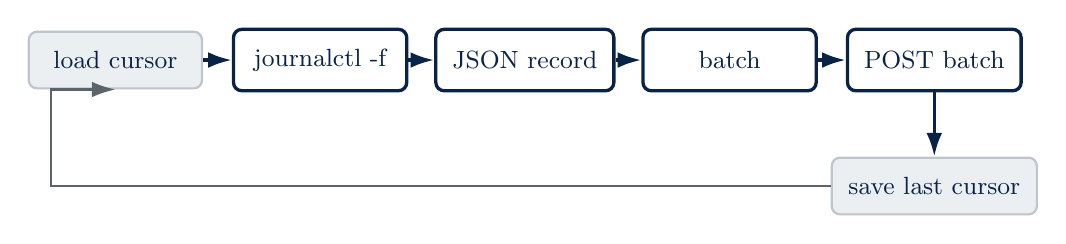
\begin{tikzpicture}[x=1cm,y=1cm]
  \node[rca/softbox,minimum width=2.2cm] (load) at (1,2.6) {load cursor};
  \node[rca/box,minimum width=2.2cm] (follow) at (3.6,2.6) {journalctl -f};
  \node[rca/box,minimum width=2.2cm] (parse) at (6.2,2.6) {JSON record};
  \node[rca/box,minimum width=2.2cm] (batch) at (8.8,2.6) {batch};
  \node[rca/box,minimum width=2.2cm] (post) at (11.4,2.6) {POST batch};
  \node[rca/softbox,minimum width=2.5cm] (save) at (11.4,1.0) {save last cursor};
  \draw[rca/arrow] (load) -- (follow);
  \draw[rca/arrow] (follow) -- (parse);
  \draw[rca/arrow] (parse) -- (batch);
  \draw[rca/arrow] (batch) -- (post);
  \draw[rca/arrow] (post) -- (save);
  \draw[rca/grayarrow] (save.west) -- ++(-9.9,0) |- (load.south);
\end{tikzpicture}
\end{frame}

\begin{frame}{Collector Watches DevStack Units}
\centering
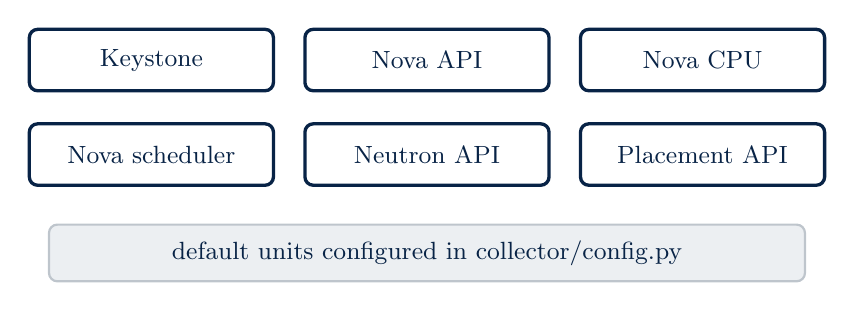
\begin{tikzpicture}[x=1cm,y=1cm]
  \node[rca/box,minimum width=3.1cm] at (2,3.2) {Keystone};
  \node[rca/box,minimum width=3.1cm] at (5.5,3.2) {Nova API};
  \node[rca/box,minimum width=3.1cm] at (9,3.2) {Nova CPU};
  \node[rca/box,minimum width=3.1cm] at (2,2.0) {Nova scheduler};
  \node[rca/box,minimum width=3.1cm] at (5.5,2.0) {Neutron API};
  \node[rca/box,minimum width=3.1cm] at (9,2.0) {Placement API};
  \node[rca/softbox,minimum width=9.6cm] at (5.5,0.75) {default units configured in collector/config.py};
\end{tikzpicture}
\end{frame}

\begin{frame}{Cursor Persistence and Deduplication}
\centering
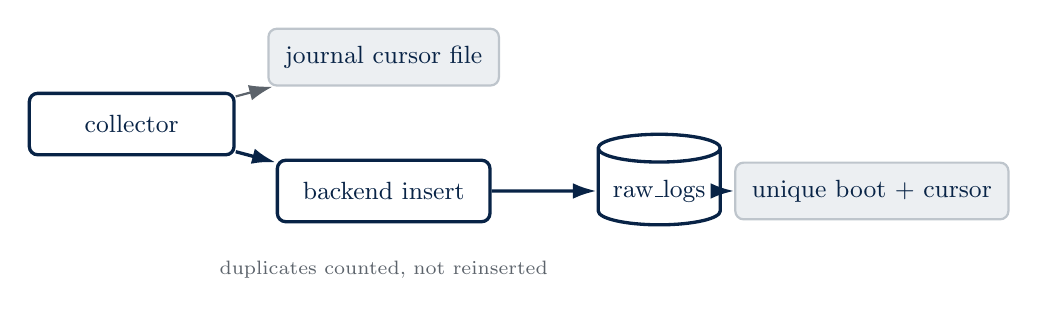
\begin{tikzpicture}[x=1cm,y=1cm]
  \node[rca/box,minimum width=2.6cm] (collector) at (1.8,2.4) {collector};
  \node[rca/softbox,minimum width=2.7cm] (cursor) at (5,3.25) {journal cursor file};
  \node[rca/box,minimum width=2.7cm] (api) at (5,1.55) {backend insert};
  \node[rca/db] (raw) at (8.5,1.55) {raw\_logs};
  \node[rca/softbox,minimum width=3.0cm] (uniq) at (11.2,1.55) {unique boot + cursor};
  \draw[rca/arrow] (collector) -- (api);
  \draw[rca/grayarrow] (collector) -- (cursor);
  \draw[rca/arrow] (api) -- (raw);
  \draw[rca/arrow] (raw) -- (uniq);
  \node[rca/tinylabel] at (5,0.55) {duplicates counted, not reinserted};
\end{tikzpicture}
\end{frame}

\begin{frame}{MongoDB Collections Map}
\centering
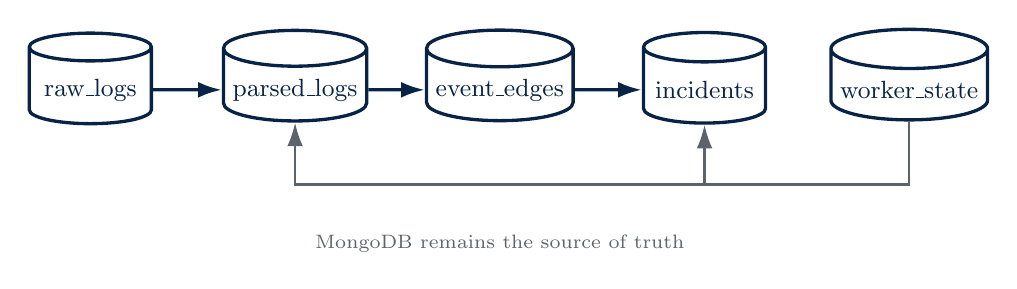
\begin{tikzpicture}[x=1cm,y=1cm]
  \node[rca/db] (raw) at (1,2.5) {raw\_logs};
  \node[rca/db] (parsed) at (3.6,2.5) {parsed\_logs};
  \node[rca/db] (edges) at (6.2,2.5) {event\_edges};
  \node[rca/db] (inc) at (8.8,2.5) {incidents};
  \node[rca/db] (state) at (11.4,2.5) {worker\_state};
  \draw[rca/arrow] (raw) -- (parsed);
  \draw[rca/arrow] (parsed) -- (edges);
  \draw[rca/arrow] (edges) -- (inc);
  \draw[rca/grayarrow] (state.south) -- ++(0,-0.8) -| (parsed.south);
  \draw[rca/grayarrow] (state.south) -- ++(0,-0.8) -| (inc.south);
  \node[rca/tinylabel] at (6.2,0.55) {MongoDB remains the source of truth};
\end{tikzpicture}
\end{frame}

\begin{frame}{raw\_logs Schema}
\centering
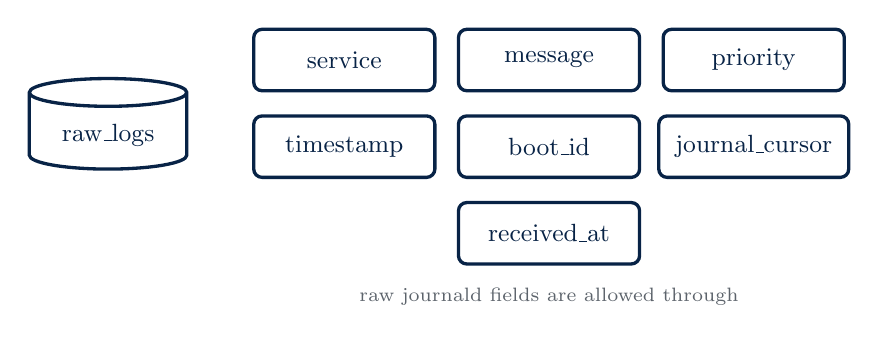
\begin{tikzpicture}[x=1cm,y=1cm]
  \node[rca/db,minimum width=2cm] at (2,2.4) {raw\_logs};
  \node[rca/box,minimum width=2.3cm] at (5,3.35) {service};
  \node[rca/box,minimum width=2.3cm] at (7.6,3.35) {message};
  \node[rca/box,minimum width=2.3cm] at (10.2,3.35) {priority};
  \node[rca/box,minimum width=2.3cm] at (5,2.25) {timestamp};
  \node[rca/box,minimum width=2.3cm] at (7.6,2.25) {boot\_id};
  \node[rca/box,minimum width=2.3cm] at (10.2,2.25) {journal\_cursor};
  \node[rca/box,minimum width=2.3cm] at (7.6,1.15) {received\_at};
  \node[rca/tinylabel] at (7.6,0.35) {raw journald fields are allowed through};
\end{tikzpicture}
\end{frame}

\begin{frame}{Backend Batch Ingest}
\centering
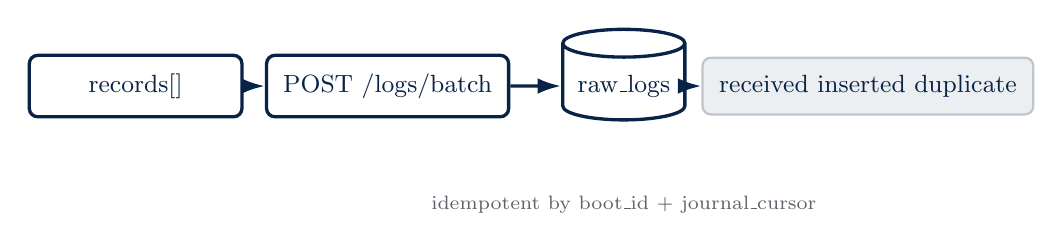
\begin{tikzpicture}[x=1cm,y=1cm]
  \node[rca/box,minimum width=2.7cm] (req) at (1.5,2.5) {records[]};
  \node[rca/box,minimum width=2.7cm] (api) at (4.7,2.5) {POST /logs/batch};
  \node[rca/db] (raw) at (7.7,2.5) {raw\_logs};
  \node[rca/softbox,minimum width=3cm] (resp) at (10.8,2.5) {received inserted duplicate};
  \draw[rca/arrow] (req) -- (api);
  \draw[rca/arrow] (api) -- (raw);
  \draw[rca/arrow] (raw) -- (resp);
  \node[rca/tinylabel] at (7.7,1.0) {idempotent by boot\_id + journal\_cursor};
\end{tikzpicture}
\end{frame}

\begin{frame}{Parser Transformation}
\centering
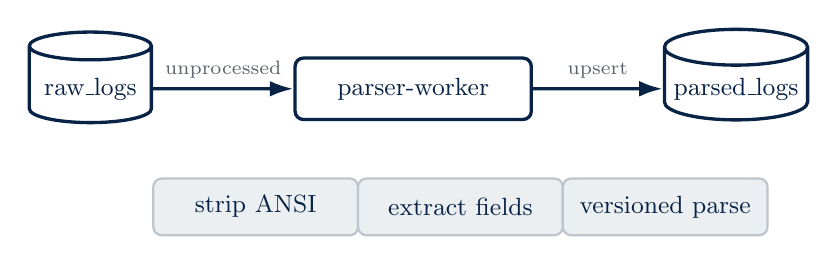
\begin{tikzpicture}[x=1cm,y=1cm]
  \node[rca/db] (raw) at (1.4,2.5) {raw\_logs};
  \node[rca/box,minimum width=3.0cm] (worker) at (5.5,2.5) {parser-worker};
  \node[rca/db] (parsed) at (9.6,2.5) {parsed\_logs};
  \draw[rca/arrow] (raw) -- node[above,rca/tinylabel] {unprocessed} (worker);
  \draw[rca/arrow] (worker) -- node[above,rca/tinylabel] {upsert} (parsed);
  \node[rca/softbox,minimum width=2.6cm] at (3.5,1.0) {strip ANSI};
  \node[rca/softbox,minimum width=2.6cm] at (6.1,1.0) {extract fields};
  \node[rca/softbox,minimum width=2.6cm] at (8.7,1.0) {versioned parse};
\end{tikzpicture}
\end{frame}

\begin{frame}{parsed\_logs Schema}
\centering
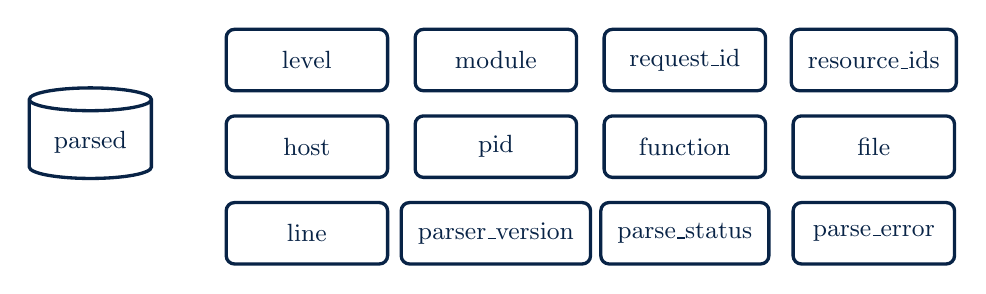
\begin{tikzpicture}[x=1cm,y=1cm]
  \node[rca/db] at (1.25,2.5) {parsed};
  \foreach \txt/\x/\y in {
    level/4/3.55,module/6.4/3.55,request\_id/8.8/3.55,
    resource\_ids/11.2/3.55,host/4/2.45,pid/6.4/2.45,
    function/8.8/2.45,file/11.2/2.45,line/4/1.35,
    parser\_version/6.4/1.35,parse\_status/8.8/1.35,parse\_error/11.2/1.35}
  {\node[rca/box,minimum width=2.05cm] at (\x,\y) {\txt};}
\end{tikzpicture}
\end{frame}

\begin{frame}{Parse Failures Are Preserved}
\centering
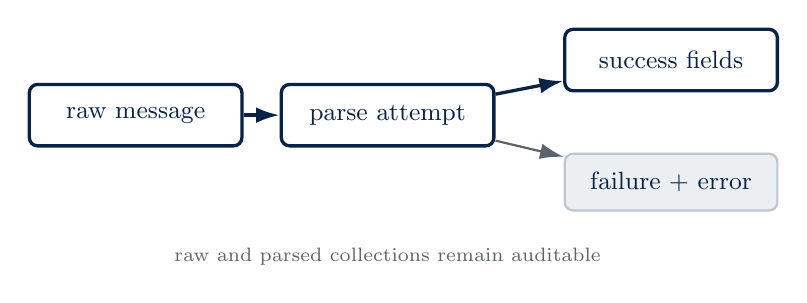
\begin{tikzpicture}[x=1cm,y=1cm]
  \node[rca/box,minimum width=2.7cm] (raw) at (1.8,2.5) {raw message};
  \node[rca/box,minimum width=2.7cm] (try) at (5,2.5) {parse attempt};
  \node[rca/box,minimum width=2.7cm] (ok) at (8.6,3.2) {success fields};
  \node[rca/softbox,minimum width=2.7cm] (fail) at (8.6,1.65) {failure + error};
  \draw[rca/arrow] (raw) -- (try);
  \draw[rca/arrow] (try) -- (ok);
  \draw[rca/grayarrow] (try) -- (fail);
  \node[rca/tinylabel] at (5,0.7) {raw and parsed collections remain auditable};
\end{tikzpicture}
\end{frame}

\begin{frame}{Correlation Graph Concept}
\centering
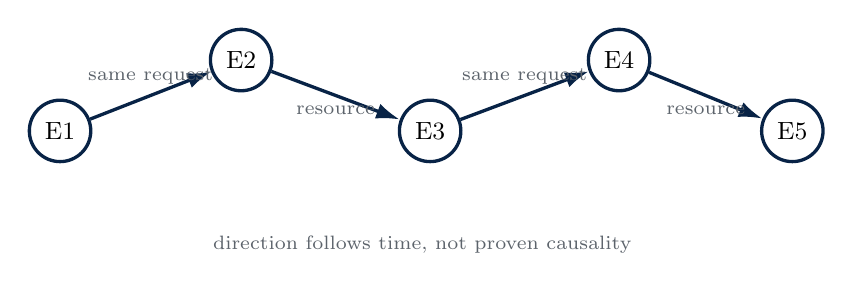
\begin{tikzpicture}[x=1cm,y=1cm]
  \node[rca/node] (a) at (2,2.3) {E1};
  \node[rca/node] (b) at (4.3,3.2) {E2};
  \node[rca/node] (c) at (6.7,2.3) {E3};
  \node[rca/node] (d) at (9.1,3.2) {E4};
  \node[rca/node] (e) at (11.3,2.3) {E5};
  \draw[rca/arrow] (a) -- node[above,rca/tinylabel] {same request} (b);
  \draw[rca/arrow] (b) -- node[below,rca/tinylabel] {resource} (c);
  \draw[rca/arrow] (c) -- node[above,rca/tinylabel] {same request} (d);
  \draw[rca/arrow] (d) -- node[below,rca/tinylabel] {resource} (e);
  \node[rca/tinylabel] at (6.6,0.85) {direction follows time, not proven causality};
\end{tikzpicture}
\end{frame}

\begin{frame}{request\_id Edge Example}
\centering
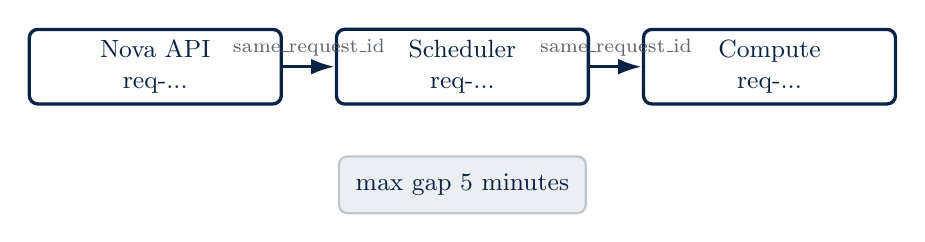
\begin{tikzpicture}[x=1cm,y=1cm]
  \node[rca/box,minimum width=3.2cm] (n1) at (2.1,2.5) {Nova API\\req-...};
  \node[rca/box,minimum width=3.2cm] (n2) at (6,2.5) {Scheduler\\req-...};
  \node[rca/box,minimum width=3.2cm] (n3) at (9.9,2.5) {Compute\\req-...};
  \draw[rca/arrow] (n1) -- node[above,rca/tinylabel] {same\_request\_id} (n2);
  \draw[rca/arrow] (n2) -- node[above,rca/tinylabel] {same\_request\_id} (n3);
  \node[rca/softbox,minimum width=3cm] at (6,1.0) {max gap 5 minutes};
\end{tikzpicture}
\end{frame}

\begin{frame}{resource\_id Edge Example}
\centering
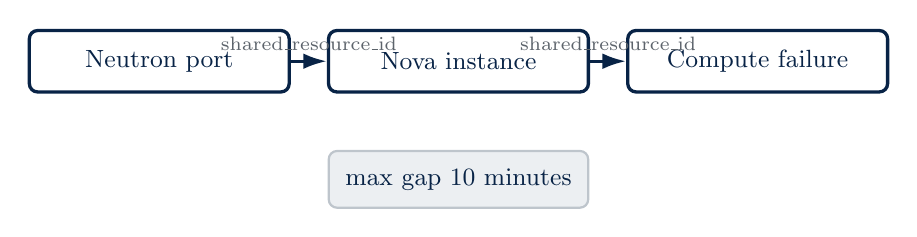
\begin{tikzpicture}[x=1cm,y=1cm]
  \node[rca/box,minimum width=3.3cm] (n1) at (2.2,2.5) {Neutron port};
  \node[rca/box,minimum width=3.3cm] (n2) at (6,2.5) {Nova instance};
  \node[rca/box,minimum width=3.3cm] (n3) at (9.8,2.5) {Compute failure};
  \draw[rca/arrow] (n1) -- node[above,rca/tinylabel] {shared\_resource\_id} (n2);
  \draw[rca/arrow] (n2) -- node[above,rca/tinylabel] {shared\_resource\_id} (n3);
  \node[rca/softbox,minimum width=3cm] at (6,1.0) {max gap 10 minutes};
\end{tikzpicture}
\end{frame}

\begin{frame}{Graph Explosion Problem}
\centering
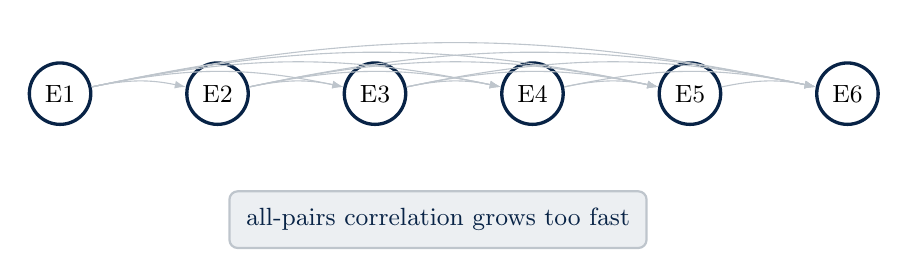
\begin{tikzpicture}[x=1cm,y=1cm]
  \foreach \i/\x in {1/1.2,2/3.2,3/5.2,4/7.2,5/9.2,6/11.2}{
    \node[rca/node] (e\i) at (\x,2.4) {E\i};
  }
  \foreach \i in {1,...,5}{
    \pgfmathtruncatemacro{\jstart}{\i+1}
    \foreach \j in {\jstart,...,6}{
      \draw[draw=RcaMidGray,thin,-{Latex[length=1.4mm,width=1.0mm]}] (e\i) to[bend left=12] (e\j);
    }
  }
  \node[rca/softbox,minimum width=4.1cm] at (6,0.8) {all-pairs correlation grows too fast};
\end{tikzpicture}
\end{frame}

\begin{frame}{Graph Explosion Fix}
\centering
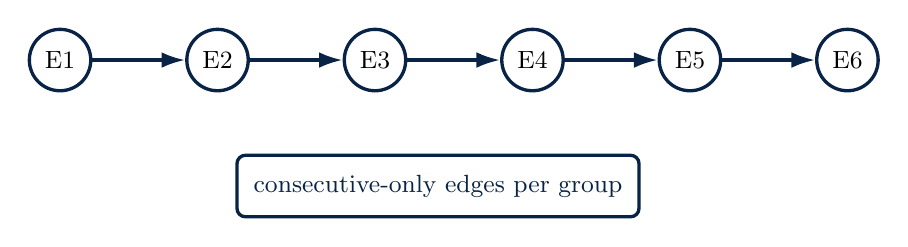
\begin{tikzpicture}[x=1cm,y=1cm]
  \foreach \i/\x in {1/1.2,2/3.2,3/5.2,4/7.2,5/9.2,6/11.2}{
    \node[rca/node] (e\i) at (\x,2.4) {E\i};
  }
  \foreach \i/\j in {1/2,2/3,3/4,4/5,5/6}{
    \draw[rca/arrow] (e\i) -- (e\j);
  }
  \node[rca/box,minimum width=4.4cm] at (6,0.8) {consecutive-only edges per group};
\end{tikzpicture}
\end{frame}

\begin{frame}{Periodic Group Skip}
\centering
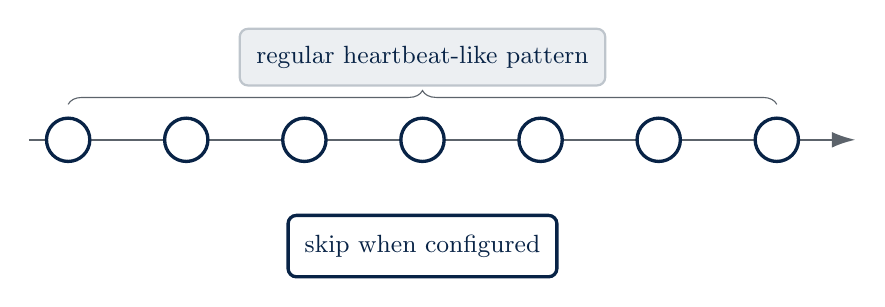
\begin{tikzpicture}[x=1cm,y=1cm]
  \draw[rca/grayarrow] (1,2.4) -- (11.5,2.4);
  \foreach \x in {1.5,3.0,4.5,6.0,7.5,9.0,10.5}{
    \node[rca/node,minimum size=0.55cm] at (\x,2.4) {};
  }
  \node[rca/softbox,minimum width=3.0cm] at (6,3.45) {regular heartbeat-like pattern};
  \node[rca/box,minimum width=3.0cm] at (6,1.05) {skip when configured};
  \draw[decorate,decoration={brace,amplitude=5pt},draw=RcaGray] (1.5,2.85) -- (10.5,2.85);
\end{tikzpicture}
\end{frame}

\begin{frame}{Correlation Worker Safeguards}
\centering
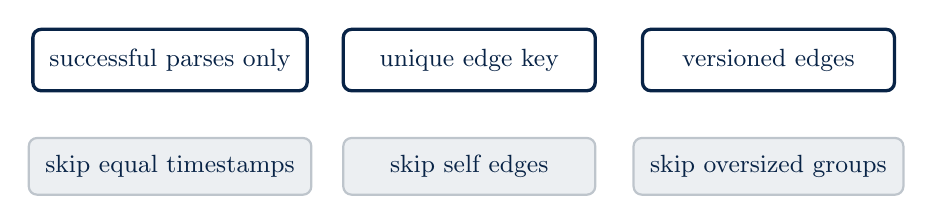
\begin{tikzpicture}[x=1cm,y=1cm]
  \node[rca/box,minimum width=3.2cm] at (2.2,2.9) {successful parses only};
  \node[rca/box,minimum width=3.2cm] at (6,2.9) {unique edge key};
  \node[rca/box,minimum width=3.2cm] at (9.8,2.9) {versioned edges};
  \node[rca/softbox,minimum width=3.2cm] at (2.2,1.55) {skip equal timestamps};
  \node[rca/softbox,minimum width=3.2cm] at (6,1.55) {skip self edges};
  \node[rca/softbox,minimum width=3.2cm] at (9.8,1.55) {skip oversized groups};
\end{tikzpicture}
\end{frame}

\begin{frame}{Incident Seed Detection Flow}
\centering
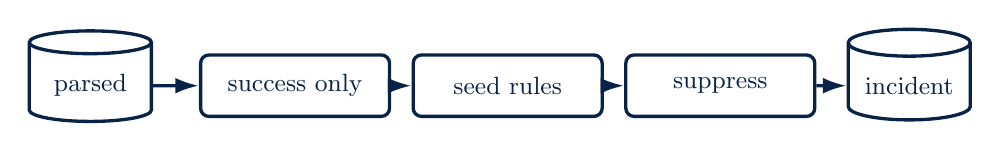
\begin{tikzpicture}[x=1cm,y=1cm]
  \node[rca/db] (p) at (1.2,2.4) {parsed};
  \node[rca/box,minimum width=2.4cm] (filter) at (3.8,2.4) {success only};
  \node[rca/box,minimum width=2.4cm] (rules) at (6.5,2.4) {seed rules};
  \node[rca/box,minimum width=2.4cm] (suppress) at (9.2,2.4) {suppress};
  \node[rca/db] (inc) at (11.6,2.4) {incident};
  \draw[rca/arrow] (p) -- (filter);
  \draw[rca/arrow] (filter) -- (rules);
  \draw[rca/arrow] (rules) -- (suppress);
  \draw[rca/arrow] (suppress) -- (inc);
\end{tikzpicture}
\end{frame}

\begin{frame}{Deterministic Seed Rules}
\centering
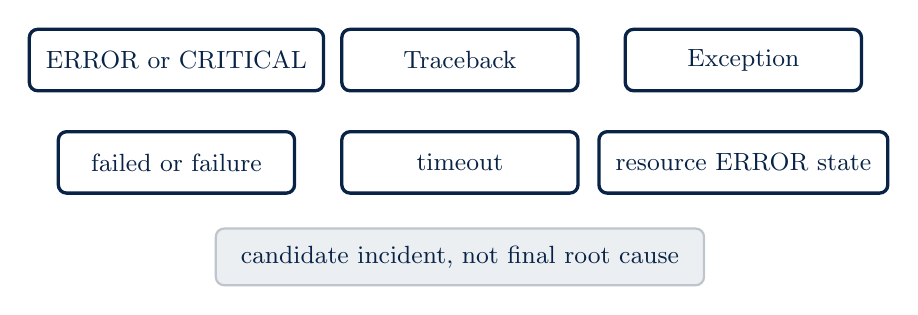
\begin{tikzpicture}[x=1cm,y=1cm]
  \foreach \txt/\x/\y in {
    ERROR or CRITICAL/3/3.3,Traceback/6.6/3.3,Exception/10.2/3.3,
    failed or failure/3/2.0,timeout/6.6/2.0,resource ERROR state/10.2/2.0}
  {\node[rca/box,minimum width=3.0cm] at (\x,\y) {\txt};}
  \node[rca/softbox,minimum width=6.2cm] at (6.6,0.8) {candidate incident, not final root cause};
\end{tikzpicture}
\end{frame}

\begin{frame}{False-Positive Suppression}
\centering
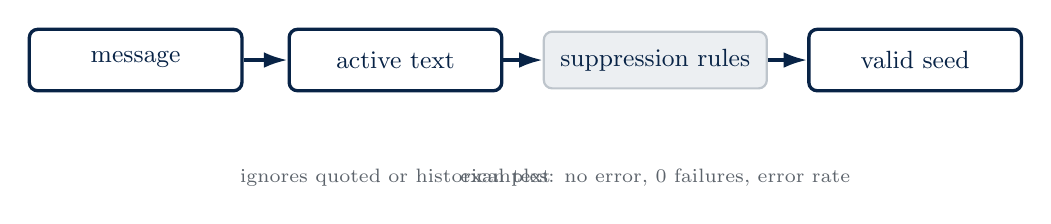
\begin{tikzpicture}[x=1cm,y=1cm]
  \node[rca/box,minimum width=2.7cm] (msg) at (1.6,2.5) {message};
  \node[rca/box,minimum width=2.7cm] (clean) at (4.9,2.5) {active text};
  \node[rca/softbox,minimum width=2.7cm] (patterns) at (8.2,2.5) {suppression rules};
  \node[rca/box,minimum width=2.7cm] (seed) at (11.5,2.5) {valid seed};
  \draw[rca/arrow] (msg) -- (clean);
  \draw[rca/arrow] (clean) -- (patterns);
  \draw[rca/arrow] (patterns) -- (seed);
  \node[rca/tinylabel] at (4.9,1.0) {ignores quoted or historical text};
  \node[rca/tinylabel] at (8.2,1.0) {examples: no error, 0 failures, error rate};
\end{tikzpicture}
\end{frame}

\begin{frame}{Incident Subgraph Traversal}
\centering
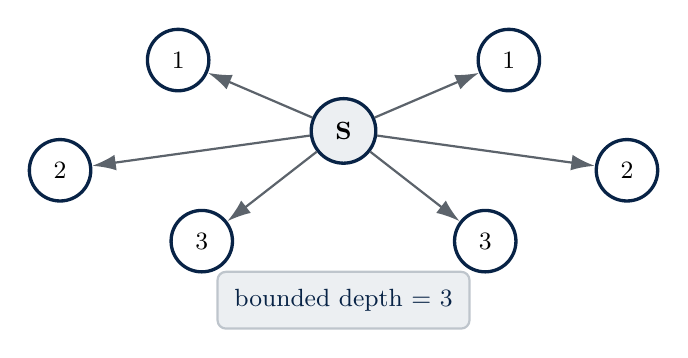
\begin{tikzpicture}[x=1cm,y=1cm]
  \node[rca/error] (s) at (6,2.5) {S};
  \node[rca/node] (a) at (3.9,3.4) {1};
  \node[rca/node] (b) at (8.1,3.4) {1};
  \node[rca/node] (c) at (2.4,2.0) {2};
  \node[rca/node] (d) at (9.6,2.0) {2};
  \node[rca/node] (e) at (4.2,1.1) {3};
  \node[rca/node] (f) at (7.8,1.1) {3};
  \foreach \x in {a,b,c,d,e,f}{\draw[rca/grayarrow] (s) -- (\x);}
  \node[rca/softbox,minimum width=3.2cm] at (6,0.35) {bounded depth = 3};
\end{tikzpicture}
\end{frame}

\begin{frame}{Incident Boundaries}
\centering
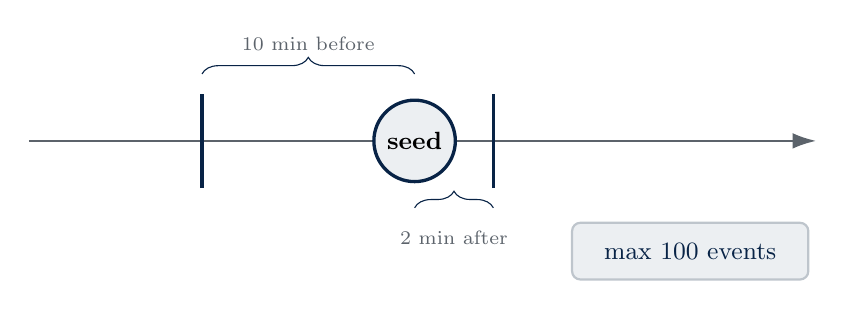
\begin{tikzpicture}[x=1cm,y=1cm]
  \draw[rca/grayarrow] (1.2,2.4) -- (11.2,2.4);
  \node[rca/error] at (6.1,2.4) {seed};
  \draw[draw=RcaNavy,very thick] (3.4,1.8) -- (3.4,3.0);
  \draw[draw=RcaNavy,very thick] (7.1,1.8) -- (7.1,3.0);
  \draw[decorate,decoration={brace,amplitude=6pt},draw=RcaNavy] (3.4,3.25) -- node[above=5pt,rca/tinylabel] {10 min before} (6.1,3.25);
  \draw[decorate,decoration={brace,amplitude=6pt},draw=RcaNavy] (6.1,1.55) -- node[below=5pt,rca/tinylabel] {2 min after} (7.1,1.55);
  \node[rca/softbox,minimum width=3.0cm] at (9.6,1.0) {max 100 events};
\end{tikzpicture}
\end{frame}

\begin{frame}{Candidate Incident Document}
\centering
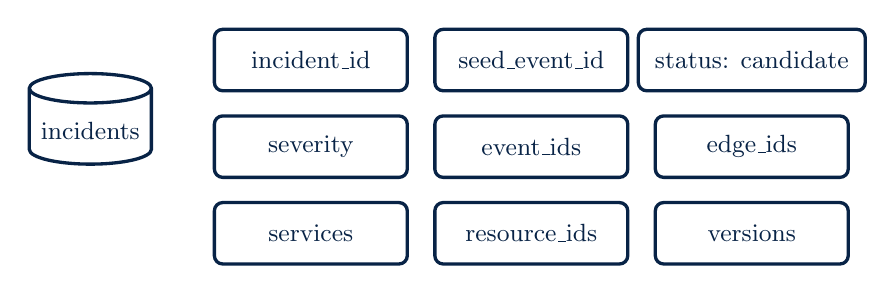
\begin{tikzpicture}[x=1cm,y=1cm]
  \node[rca/db] at (1.4,2.5) {incidents};
  \foreach \txt/\x/\y in {
    incident\_id/4.2/3.4,seed\_event\_id/7/3.4,status: candidate/9.8/3.4,
    severity/4.2/2.3,event\_ids/7/2.3,edge\_ids/9.8/2.3,
    services/4.2/1.2,resource\_ids/7/1.2,versions/9.8/1.2}
  {\node[rca/box,minimum width=2.45cm] at (\x,\y) {\txt};}
\end{tikzpicture}
\end{frame}

\begin{frame}{Enrichment Pipeline}
\centering
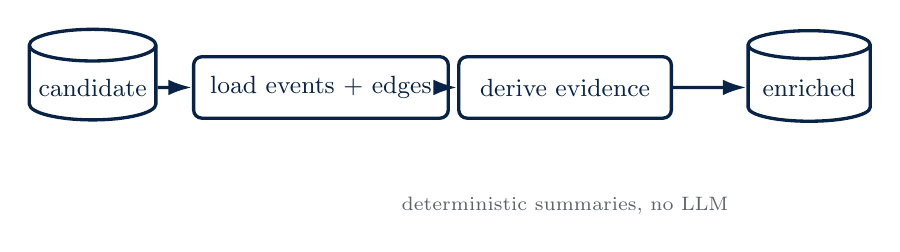
\begin{tikzpicture}[x=1cm,y=1cm]
  \node[rca/db] (inc) at (1.3,2.5) {candidate};
  \node[rca/box,minimum width=2.7cm] (load) at (4.2,2.5) {load events + edges};
  \node[rca/box,minimum width=2.7cm] (derive) at (7.3,2.5) {derive evidence};
  \node[rca/db] (en) at (10.4,2.5) {enriched};
  \draw[rca/arrow] (inc) -- (load);
  \draw[rca/arrow] (load) -- (derive);
  \draw[rca/arrow] (derive) -- (en);
  \node[rca/tinylabel] at (7.3,1.0) {deterministic summaries, no LLM};
\end{tikzpicture}
\end{frame}

\begin{frame}{Enriched Incident Timeline}
\centering
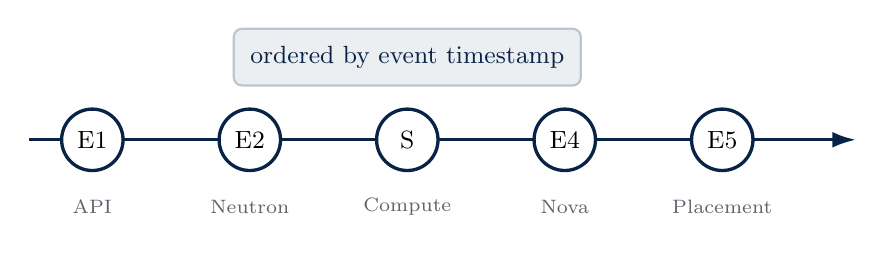
\begin{tikzpicture}[x=1cm,y=1cm]
  \draw[rca/arrow] (1.2,2.4) -- (11.7,2.4);
  \foreach \x/\lab/\svc in {2/E1/API,4/E2/Neutron,6/S/Compute,8/E4/Nova,10/E5/Placement}{
    \node[rca/node] at (\x,2.4) {\lab};
    \node[rca/tinylabel] at (\x,1.55) {\svc};
  }
  \node[rca/softbox,minimum width=3.2cm] at (6,3.45) {ordered by event timestamp};
\end{tikzpicture}
\end{frame}

\begin{frame}{Enrichment Adds Investigation Fields}
\centering
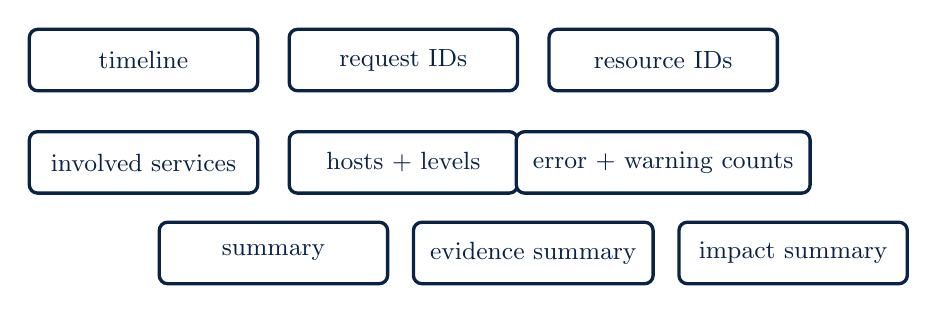
\begin{tikzpicture}[x=1cm,y=1cm]
  \foreach \txt/\x/\y in {
    timeline/2.2/3.3,request IDs/5.5/3.3,resource IDs/8.8/3.3,
    involved services/2.2/2.0,hosts + levels/5.5/2.0,error + warning counts/8.8/2.0,
    summary/3.85/0.85,evidence summary/7.15/0.85,impact summary/10.45/0.85}
  {\node[rca/box,minimum width=2.9cm] at (\x,\y) {\txt};}
\end{tikzpicture}
\end{frame}

\begin{frame}{What the Current System Does Not Claim}
\centering
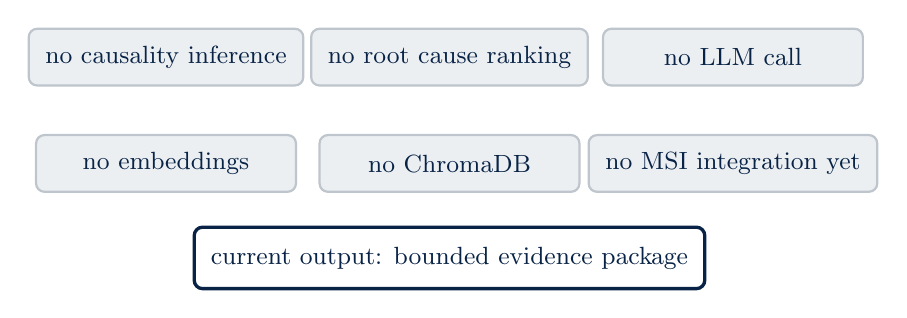
\begin{tikzpicture}[x=1cm,y=1cm]
  \node[rca/softbox,minimum width=3.3cm] at (2.5,3.2) {no causality inference};
  \node[rca/softbox,minimum width=3.3cm] at (6.1,3.2) {no root cause ranking};
  \node[rca/softbox,minimum width=3.3cm] at (9.7,3.2) {no LLM call};
  \node[rca/softbox,minimum width=3.3cm] at (2.5,1.85) {no embeddings};
  \node[rca/softbox,minimum width=3.3cm] at (6.1,1.85) {no ChromaDB};
  \node[rca/softbox,minimum width=3.3cm] at (9.7,1.85) {no MSI integration yet};
  \node[rca/box,minimum width=5.4cm] at (6.1,0.65) {current output: bounded evidence package};
\end{tikzpicture}
\end{frame}

\begin{frame}{Full Current End-to-End Pipeline}
\centering
\resizebox{\textwidth}{!}{%

\begin{tikzpicture}[x=1cm,y=1cm]
  \node[rca/box] (j) at (0,2.2) {journald};
  \node[rca/box] (c) at (1.9,2.2) {collector};
  \node[rca/box] (b) at (3.8,2.2) {backend};
  \node[rca/db] (raw) at (5.6,2.2) {raw\_logs};
  \node[rca/box] (p) at (7.5,2.2) {parser};
  \node[rca/db] (pl) at (9.4,2.2) {parsed};
  \node[rca/box] (cw) at (11.3,2.2) {correlate};
  \node[rca/db] (ed) at (13.2,2.2) {edges};
  \node[rca/box] (iw) at (15.1,2.2) {incident};
  \node[rca/db] (in) at (17.0,2.2) {incidents};
  \node[rca/box] (ew) at (18.9,2.2) {enrich};
  \node[rca/db] (en) at (20.8,2.2) {enriched};
  \foreach \a/\bb in {j/c,c/b,b/raw,raw/p,p/pl,pl/cw,cw/ed,ed/iw,iw/in,in/ew,ew/en}{\draw[rca/arrow] (\a) -- (\bb);}
\end{tikzpicture}}
\end{frame}

\begin{frame}{Current Pipeline Responsibilities}
\centering
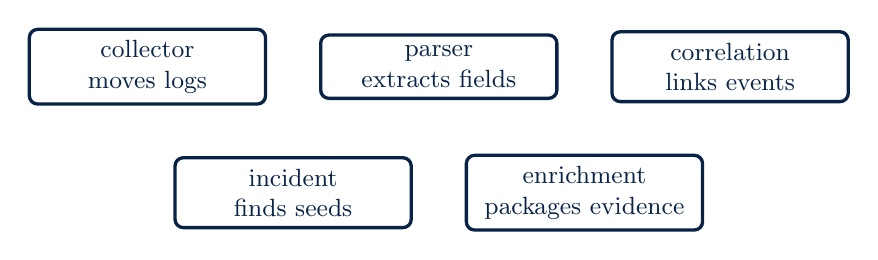
\begin{tikzpicture}[x=1cm,y=1cm]
  \node[rca/box,minimum width=3.0cm] at (2.3,3.2) {collector\\moves logs};
  \node[rca/box,minimum width=3.0cm] at (6.0,3.2) {parser\\extracts fields};
  \node[rca/box,minimum width=3.0cm] at (9.7,3.2) {correlation\\links events};
  \node[rca/box,minimum width=3.0cm] at (4.15,1.6) {incident\\finds seeds};
  \node[rca/box,minimum width=3.0cm] at (7.85,1.6) {enrichment\\packages evidence};
\end{tikzpicture}
\end{frame}

\begin{frame}{Future RAG Stage}
\centering
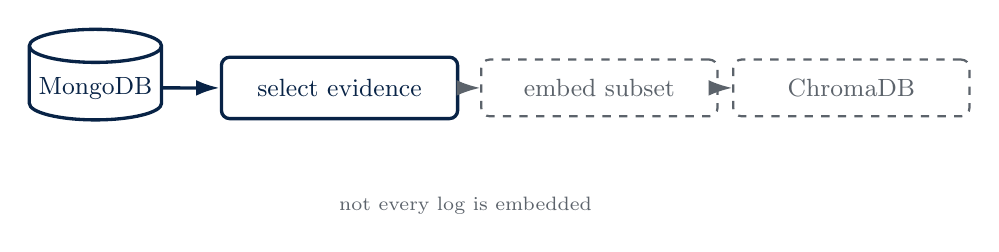
\begin{tikzpicture}[x=1cm,y=1cm]
  \node[rca/db] (mongo) at (1.5,2.5) {MongoDB};
  \node[rca/box,minimum width=3.0cm] (select) at (4.6,2.5) {select evidence};
  \node[rca/future,minimum width=3.0cm] (embed) at (7.9,2.5) {embed subset};
  \node[rca/future,minimum width=3.0cm] (chroma) at (11.1,2.5) {ChromaDB};
  \draw[rca/arrow] (mongo) -- (select);
  \draw[rca/dasharrow] (select) -- (embed);
  \draw[rca/dasharrow] (embed) -- (chroma);
  \node[rca/tinylabel] at (6.2,1.0) {not every log is embedded};
\end{tikzpicture}
\end{frame}

\begin{frame}{Future Embedding Policy}
\centering
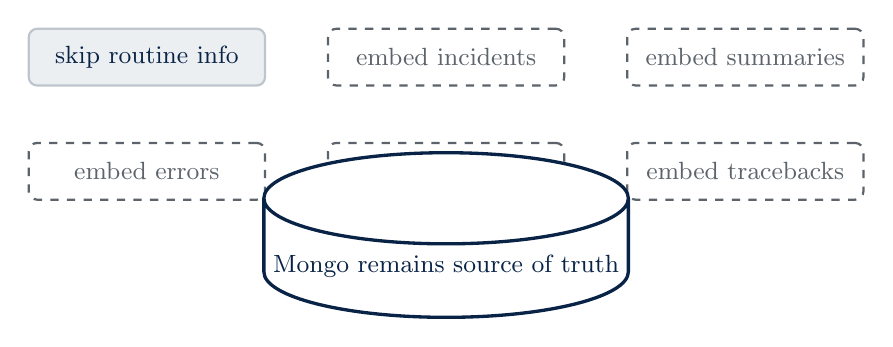
\begin{tikzpicture}[x=1cm,y=1cm]
  \node[rca/softbox,minimum width=3.0cm] at (2.2,3.2) {skip routine info};
  \node[rca/future,minimum width=3.0cm] at (6,3.2) {embed incidents};
  \node[rca/future,minimum width=3.0cm] at (9.8,3.2) {embed summaries};
  \node[rca/future,minimum width=3.0cm] at (2.2,1.75) {embed errors};
  \node[rca/future,minimum width=3.0cm] at (6,1.75) {embed warnings};
  \node[rca/future,minimum width=3.0cm] at (9.8,1.75) {embed tracebacks};
  \node[rca/db] at (6,0.55) {Mongo remains source of truth};
\end{tikzpicture}
\end{frame}

\begin{frame}{Future MSI Embedding Topology}
\centering
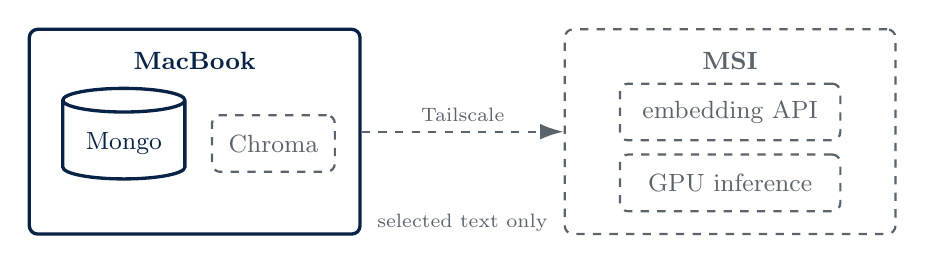
\begin{tikzpicture}[x=1cm,y=1cm]
  \node[rca/box,minimum width=4.2cm,minimum height=2.6cm] (mac) at (3,2.4) {};
  \node[rca/title] at (3,3.3) {MacBook};
  \node[rca/db] at (2.1,2.25) {Mongo};
  \node[rca/future] at (4,2.25) {Chroma};
  \node[rca/future,minimum width=4.2cm,minimum height=2.6cm] (msi) at (9.8,2.4) {};
  \node[rca/title,text=RcaGray] at (9.8,3.3) {MSI};
  \node[rca/future,minimum width=2.8cm] at (9.8,2.65) {embedding API};
  \node[rca/future,minimum width=2.8cm] at (9.8,1.75) {GPU inference};
  \draw[rca/dasharrow] (mac) -- node[above,rca/tinylabel] {Tailscale} (msi);
  \node[rca/tinylabel] at (6.4,1.25) {selected text only};
\end{tikzpicture}
\end{frame}

\begin{frame}{Future Ollama RCA Generation}
\centering
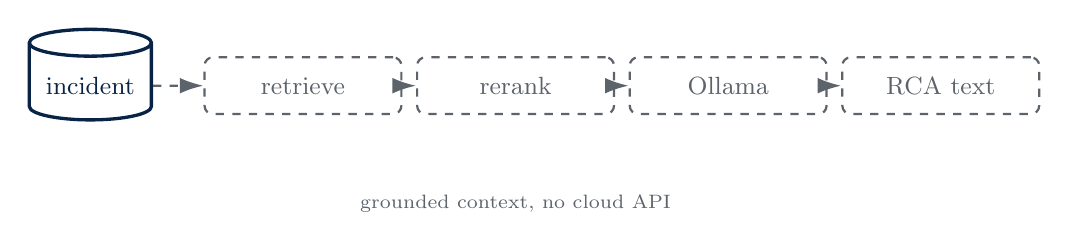
\begin{tikzpicture}[x=1cm,y=1cm]
  \node[rca/db] (inc) at (1.2,2.5) {incident};
  \node[rca/future,minimum width=2.5cm] (ret) at (3.9,2.5) {retrieve};
  \node[rca/future,minimum width=2.5cm] (rank) at (6.6,2.5) {rerank};
  \node[rca/future,minimum width=2.5cm] (ollama) at (9.3,2.5) {Ollama};
  \node[rca/future,minimum width=2.5cm] (out) at (12,2.5) {RCA text};
  \draw[rca/dasharrow] (inc) -- (ret);
  \draw[rca/dasharrow] (ret) -- (rank);
  \draw[rca/dasharrow] (rank) -- (ollama);
  \draw[rca/dasharrow] (ollama) -- (out);
  \node[rca/tinylabel] at (6.6,1.0) {grounded context, no cloud API};
\end{tikzpicture}
\end{frame}

\begin{frame}{Future Local Privacy Boundary}
\centering
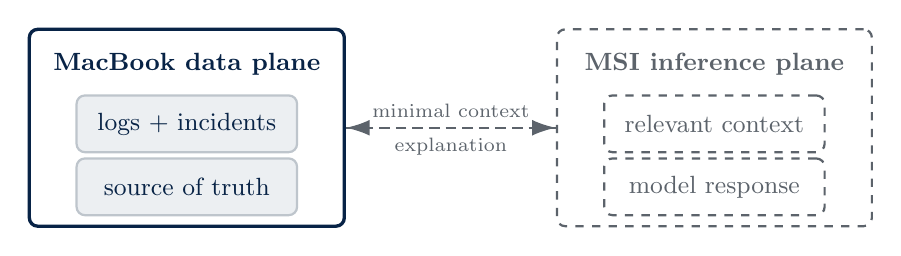
\begin{tikzpicture}[x=1cm,y=1cm]
  \node[rca/box,minimum width=4cm,minimum height=2.5cm] (mac) at (3,2.4) {};
  \node[rca/title] at (3,3.2) {MacBook data plane};
  \node[rca/softbox,minimum width=2.8cm] at (3,2.45) {logs + incidents};
  \node[rca/softbox,minimum width=2.8cm] at (3,1.65) {source of truth};
  \node[rca/future,minimum width=4cm,minimum height=2.5cm] (msi) at (9.7,2.4) {};
  \node[rca/title,text=RcaGray] at (9.7,3.2) {MSI inference plane};
  \node[rca/future,minimum width=2.8cm] at (9.7,2.45) {relevant context};
  \node[rca/future,minimum width=2.8cm] at (9.7,1.65) {model response};
  \draw[rca/dasharrow] (mac) -- node[above,rca/tinylabel] {minimal context} (msi);
  \draw[rca/dasharrow] (msi) -- node[below,rca/tinylabel] {explanation} (mac);
\end{tikzpicture}
\end{frame}

\begin{frame}{Future Horizon RCA Copilot}
\centering
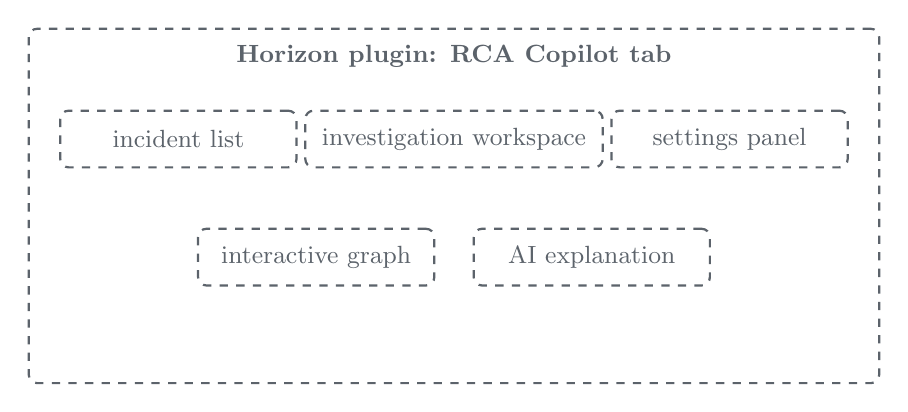
\begin{tikzpicture}[x=1cm,y=1cm]
  \node[rca/future,minimum width=10.8cm,minimum height=4.5cm] at (6,2.35) {};
  \node[rca/title,text=RcaGray] at (6,4.25) {Horizon plugin: RCA Copilot tab};
  \node[rca/future,minimum width=3.0cm] at (2.5,3.2) {incident list};
  \node[rca/future,minimum width=3.0cm] at (6,3.2) {investigation workspace};
  \node[rca/future,minimum width=3.0cm] at (9.5,3.2) {settings panel};
  \node[rca/future,minimum width=3.0cm] at (4.25,1.7) {interactive graph};
  \node[rca/future,minimum width=3.0cm] at (7.75,1.7) {AI explanation};
\end{tikzpicture}
\end{frame}

\begin{frame}{Future UI Architecture}
\centering
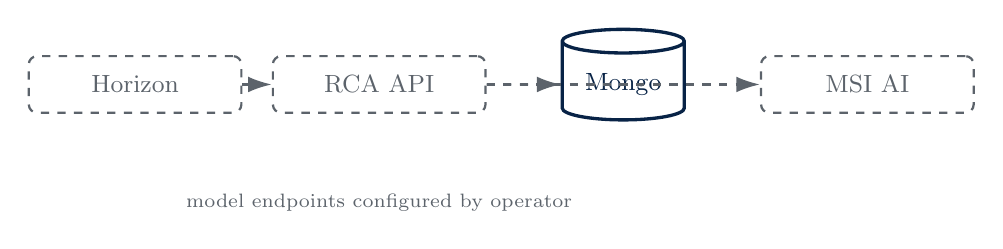
\begin{tikzpicture}[x=1cm,y=1cm]
  \node[rca/future,minimum width=2.7cm] (h) at (1.5,2.5) {Horizon};
  \node[rca/future,minimum width=2.7cm] (api) at (4.6,2.5) {RCA API};
  \node[rca/db] (mongo) at (7.7,2.5) {Mongo};
  \node[rca/future,minimum width=2.7cm] (ai) at (10.8,2.5) {MSI AI};
  \draw[rca/dasharrow] (h) -- (api);
  \draw[rca/dasharrow] (api) -- (mongo);
  \draw[rca/dasharrow] (api) -- (ai);
  \node[rca/tinylabel] at (4.6,1.0) {model endpoints configured by operator};
\end{tikzpicture}
\end{frame}

\begin{frame}{Roadmap}
\centering
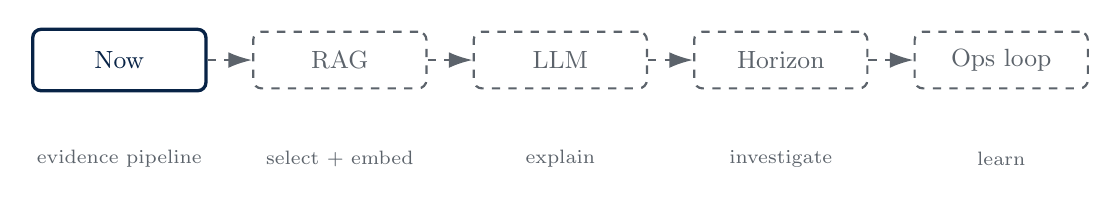
\begin{tikzpicture}[x=1cm,y=1cm]
  \node[rca/box,minimum width=2.2cm] (now) at (1.5,2.5) {Now};
  \node[rca/future,minimum width=2.2cm] (rag) at (4.3,2.5) {RAG};
  \node[rca/future,minimum width=2.2cm] (llm) at (7.1,2.5) {LLM};
  \node[rca/future,minimum width=2.2cm] (ui) at (9.9,2.5) {Horizon};
  \node[rca/future,minimum width=2.2cm] (ops) at (12.7,2.5) {Ops loop};
  \foreach \a/\b in {now/rag,rag/llm,llm/ui,ui/ops}{\draw[rca/dasharrow] (\a) -- (\b);}
  \node[rca/tinylabel] at (1.5,1.25) {evidence pipeline};
  \node[rca/tinylabel] at (4.3,1.25) {select + embed};
  \node[rca/tinylabel] at (7.1,1.25) {explain};
  \node[rca/tinylabel] at (9.9,1.25) {investigate};
  \node[rca/tinylabel] at (12.7,1.25) {learn};
\end{tikzpicture}
\end{frame}

\begin{frame}{Final Vision}
\centering
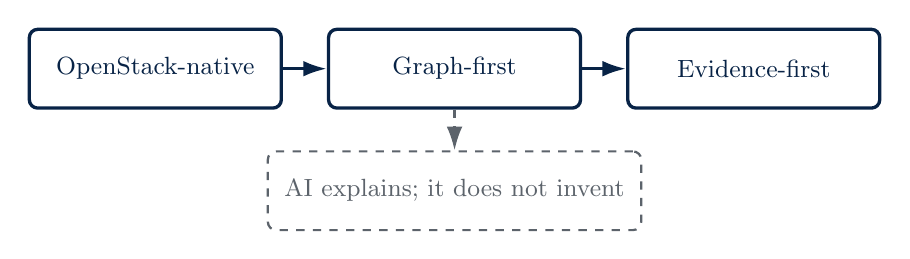
\begin{tikzpicture}[x=1cm,y=1cm]
  \node[rca/box,minimum width=3.2cm,minimum height=1.0cm] (native) at (2.2,2.8) {OpenStack-native};
  \node[rca/box,minimum width=3.2cm,minimum height=1.0cm] (graph) at (6,2.8) {Graph-first};
  \node[rca/box,minimum width=3.2cm,minimum height=1.0cm] (evidence) at (9.8,2.8) {Evidence-first};
  \node[rca/future,minimum width=4.6cm,minimum height=1.0cm] (ai) at (6,1.25) {AI explains; it does not invent};
  \draw[rca/arrow] (native) -- (graph);
  \draw[rca/arrow] (graph) -- (evidence);
  \draw[rca/dasharrow] (graph) -- (ai);
\end{tikzpicture}
\end{frame}

\begin{frame}{Takeaway}
\centering
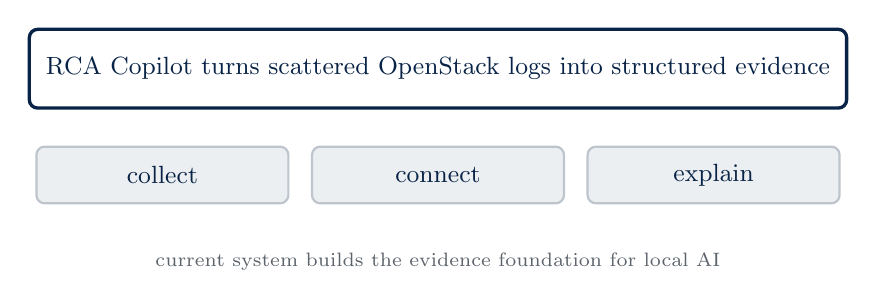
\begin{tikzpicture}[x=1cm,y=1cm]
  \node[rca/box,minimum width=9.8cm,minimum height=1.0cm] at (6,3.1) {RCA Copilot turns scattered OpenStack logs into structured evidence};
  \node[rca/softbox,minimum width=3.2cm] at (2.5,1.75) {collect};
  \node[rca/softbox,minimum width=3.2cm] at (6,1.75) {connect};
  \node[rca/softbox,minimum width=3.2cm] at (9.5,1.75) {explain};
  \node[rca/tinylabel] at (6,0.65) {current system builds the evidence foundation for local AI};
\end{tikzpicture}
\end{frame}

\end{document}
